
\chapter{Popis zařízení:}
		Zařízení se skládá z následujících základních částí: STŮL, RACK, INTERFACE, vyměnitelných ADAPTÉRŮ
		a ostatních zařízení připojených do rackového PC. Zařízení je určeno k programování a testování
		desek plošných spojů (dále označováno jako DUT). DUT se vkládá do ADAPTÉRU, kde je nakontaktováno pomocí mechanického
		zavírání a testovacích jehel. Proces je do jisté míry automatizován řídícím softwarem,
		který je popsán v kapitole software. Software předává obsluze pokyny a informace pomocí textu na monitoru. 
		
		\begin{figure}[ht!]
			\centering
			\includegraphics[height = 0.74\textheight]{obrazky/Zapojeni.png}
			\caption{Blokový diagram zapojení pracoviště}
            \label{fig:Blokový diagram zapojení pracoviště}
		\end{figure}
\clearpage
	\section{Stůl}
	Celý systém je zabudován do stolu. Stůl disponuje možností nastavitelnosti výšky celé konstrukce a sklonu desky,
	do které je upevněn INTERFACE a ADAPTÉR. Do stolu je přivedeno napětí 230V,
	které je dále rozvedeno přes proudový chránič do zásuvek pod stolem a RACKU.\\

	\begin{figure}[ht!]
		\begin{minipage}{0.49\textwidth}
			\vspace{-3.3cm}
			\textbf{Nastavení výšky:}\\\\
			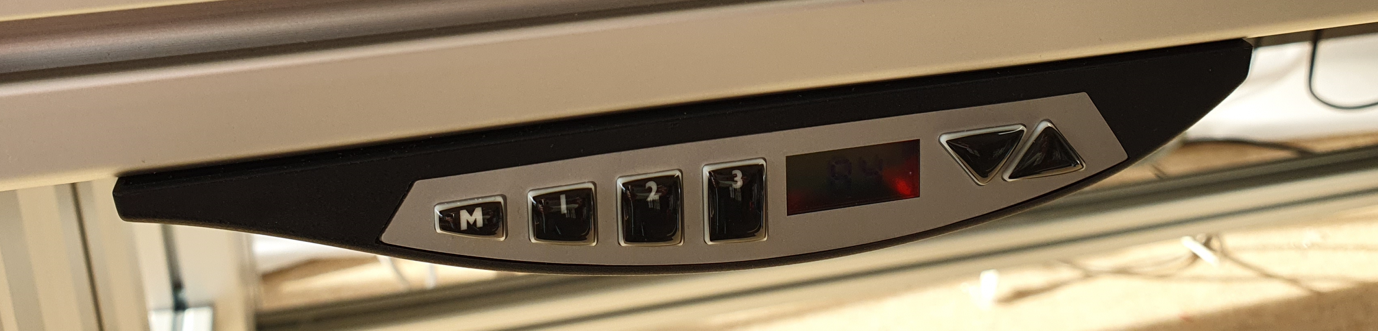
\includegraphics[width = 0.9\textwidth]{obrazky/vyska.png}
            \caption{Nastavení výšky stolu}
			
		\end{minipage}
		\begin{minipage}{0.49\textwidth}
			\textbf{Nastavení sklonu:}\\\\
			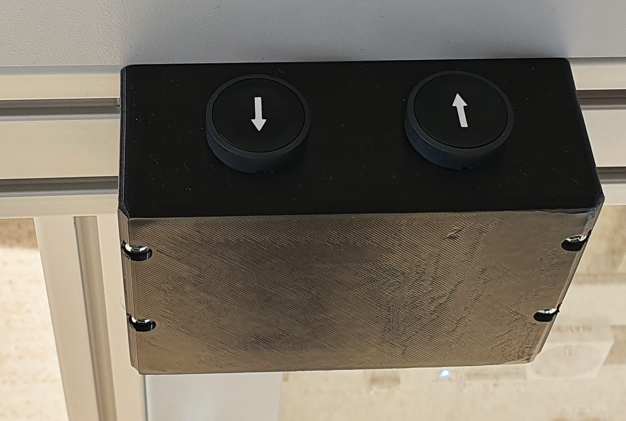
\includegraphics[width = 0.9\textwidth]{obrazky/sklon.png}
            \caption{Nastavení sklonu stolu}
			
		\end{minipage}
	\end{figure}

	\section{Rack}
	Úkolem RACK je poskytnou napájení celému systému pomocí několika galvanicky oddělených zdrojů napětí (viz schéma el. zapojení).
	Je zde umístěn i programovatelný zdroj GWINSTEK GPP-2323 jehož výstupy (kanál 1 a 2)
	jsou vyvedeny do svorek na přední části RACKU pro potřeby kalibrace.
	Dále obsahuje servisní zásuvku a bezpečnostní prvky jako vypínací tlačítko, jističe a proudový chránič.
	Dále je zde umístěn počítač, který celý systém řídí pomocí softwaru popsaného v kapitole SOFTWARE.
    Rack je možné uzamykat pomocí zámku na klíč.

	\section{Interface}
	V interface je umístěna hlavní řídící deska ARRIGO která ovládá a monituruje stav zařízení
	(spínání relátek, identifikace připojeného adaptéru, kontrola zavření víka apod.).
	Dále je zde umístěno několik programátorů (FLASHRUNNER, Segger Flasher PRO, ASIPROG a SCANBOOSTERII boundary scan).
	Za účelem externího programování (bez adaptéru) je vyveden výstup z FLASHRUNNER do konektoru CANNON 25
    na krabici (viz schéma el. zapojení).

	\section{Adaptér}
	Do interface je možno připojit adaptér pomocí propojení přes 170 pinový blok a zaaretování mechanickou pákou.
	ADAPTÉR obsahuje jehlové pole určené k nakontaktování na testpointy DUT,
	mechanické zavírání s detekcí správného založení desky a frézku ke značení testovaných desek.
	Každý adaptér dále obsahuje minimálně jednu relé kartu pro přivedení příslušných signálů na testpointy.
    V současné době je k dispozici 5 připojitelných adaptérů, které jsou schopny otestovat
    22 různých DUT.\\

    V některých složitějších adaptérech lze najít hardware dedikovaný danému provedení DUT. U některých DUT se například
    pro zákaznické čipy používá speciální přídavný hardware. Dále je v některých adaptérech možné najít optické vlákna
    s označením neohýbat. Každý adaptér má dále ve své přední části umístěny signalizační LED.

	\begin{figure}[ht!]
		\begin{minipage}{0.49\textwidth}
			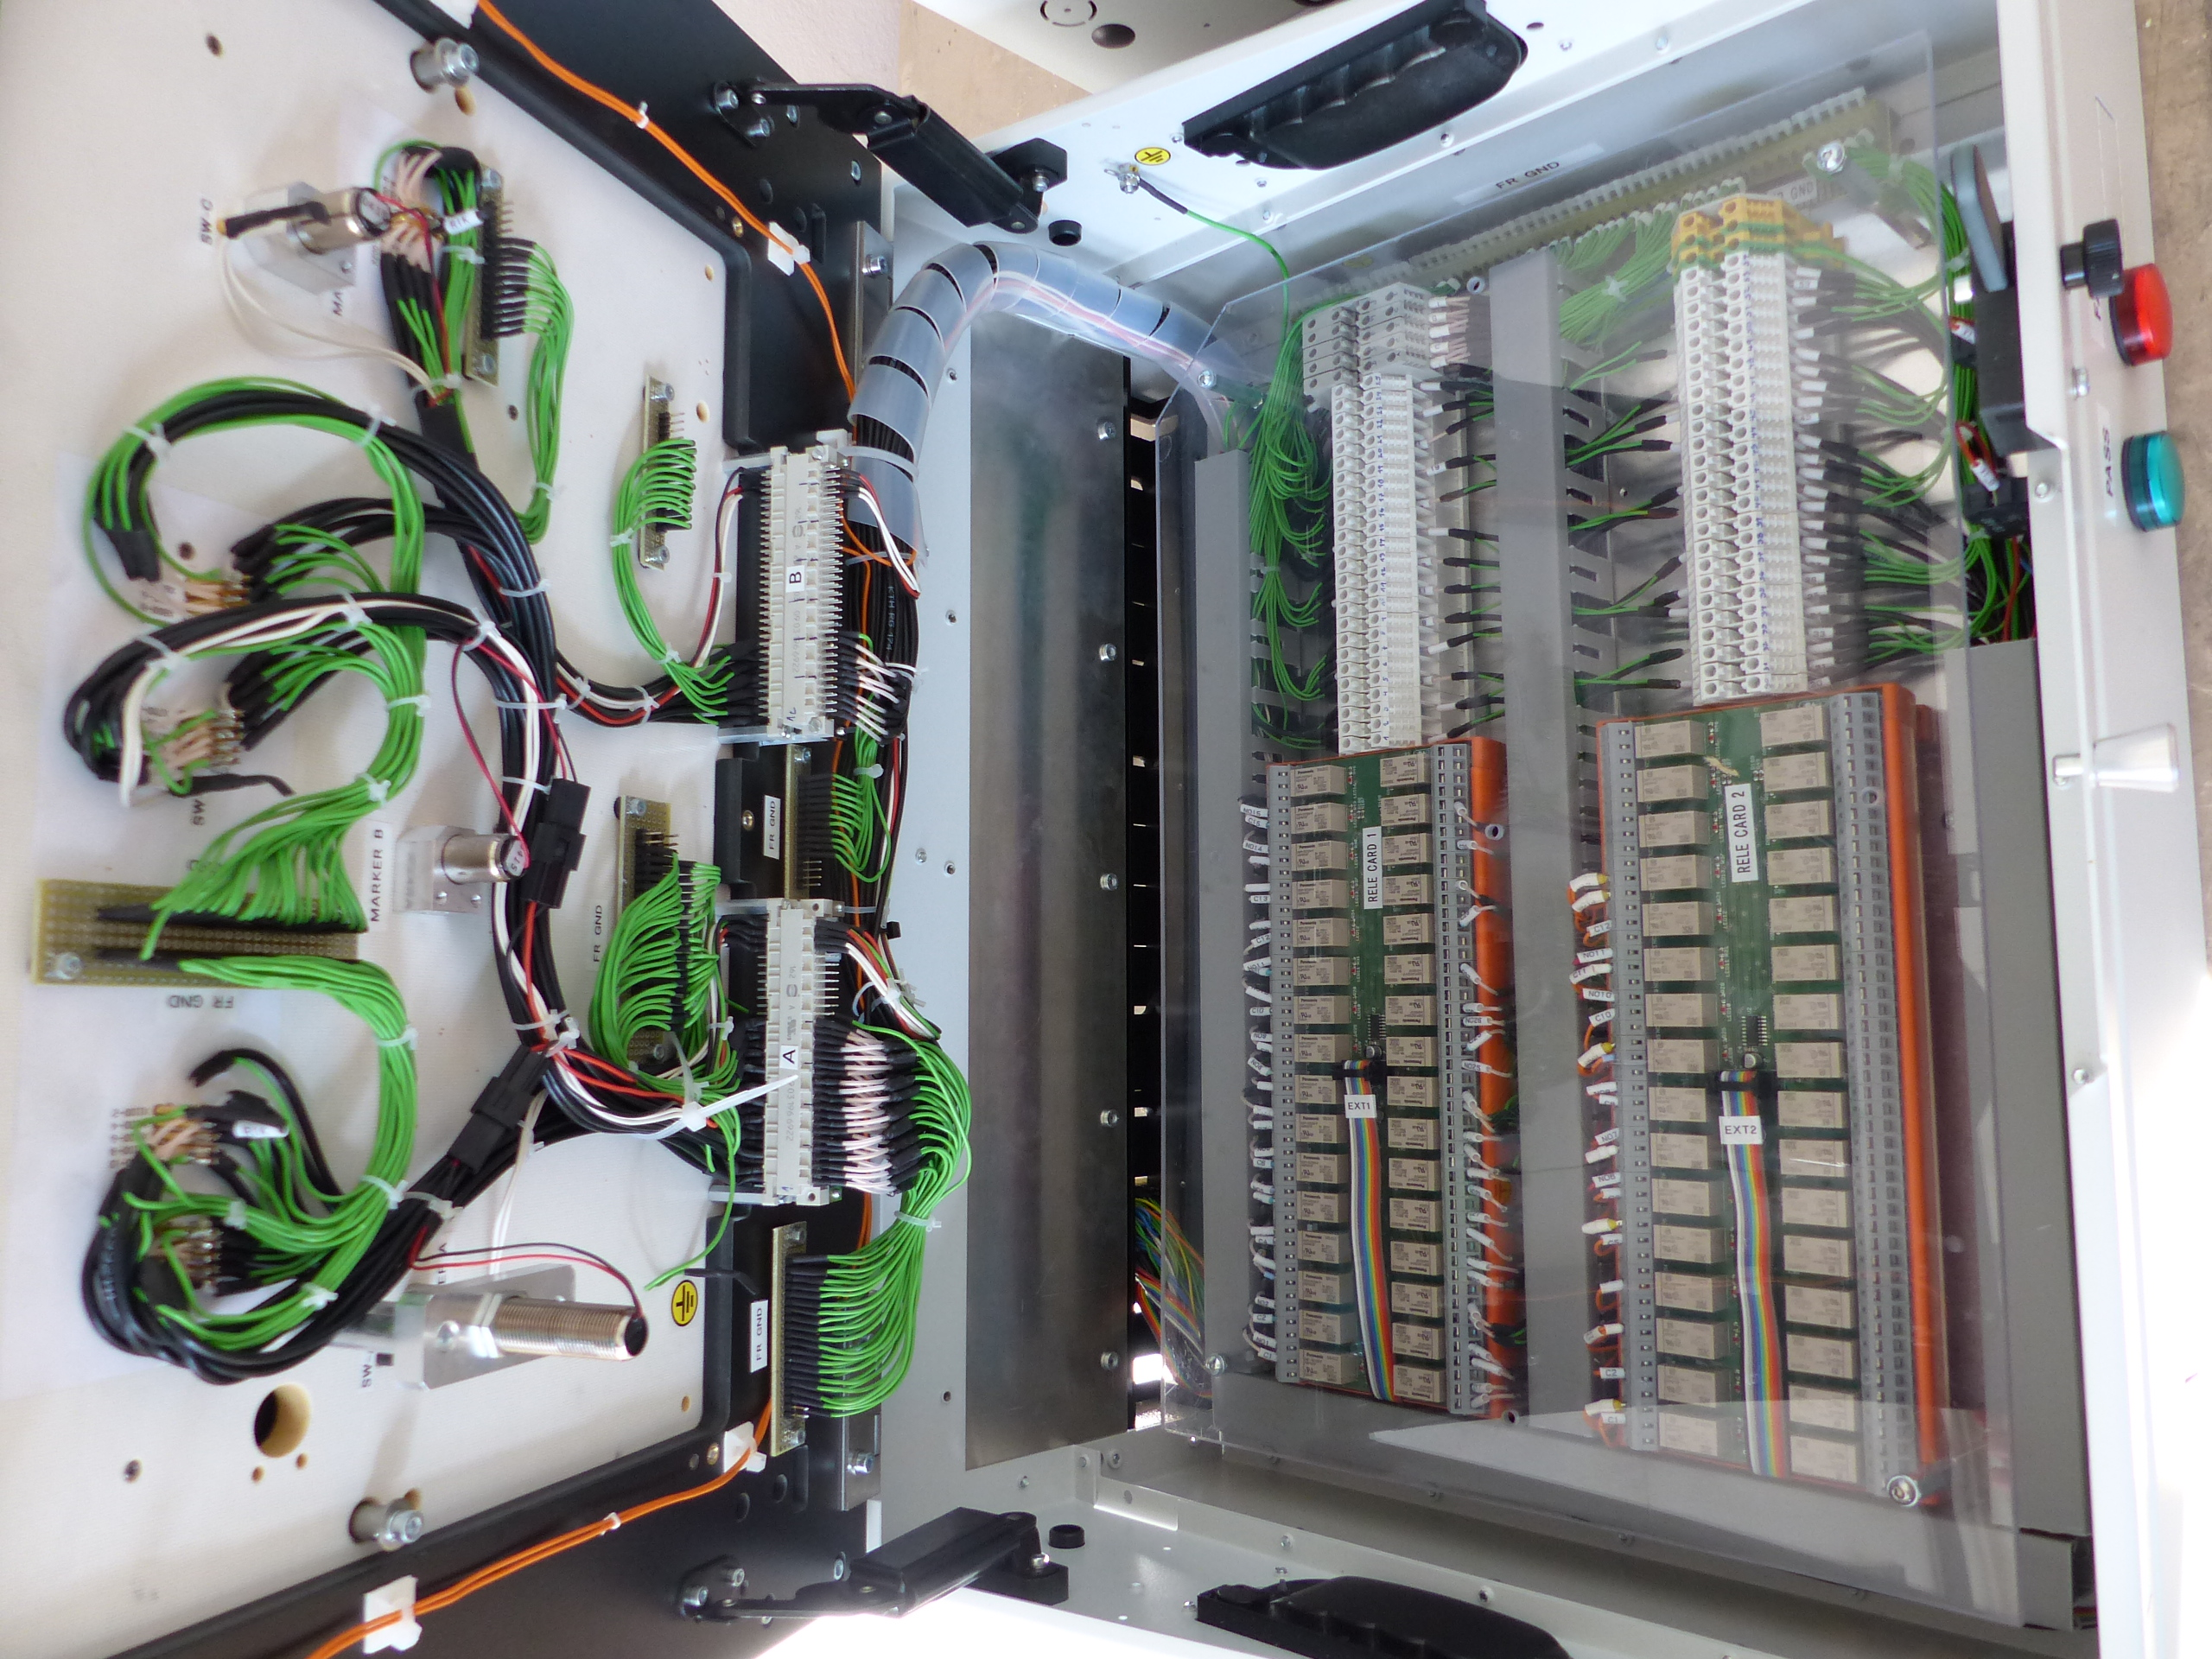
\includegraphics[width = \textwidth ,angle = -90]{obrazky/ADAPTER_INSIGHT.jpg}
            \caption{Vnitřní zapojení adaptéru}
			
		\end{minipage}
		\begin{minipage}{0.49\textwidth}
			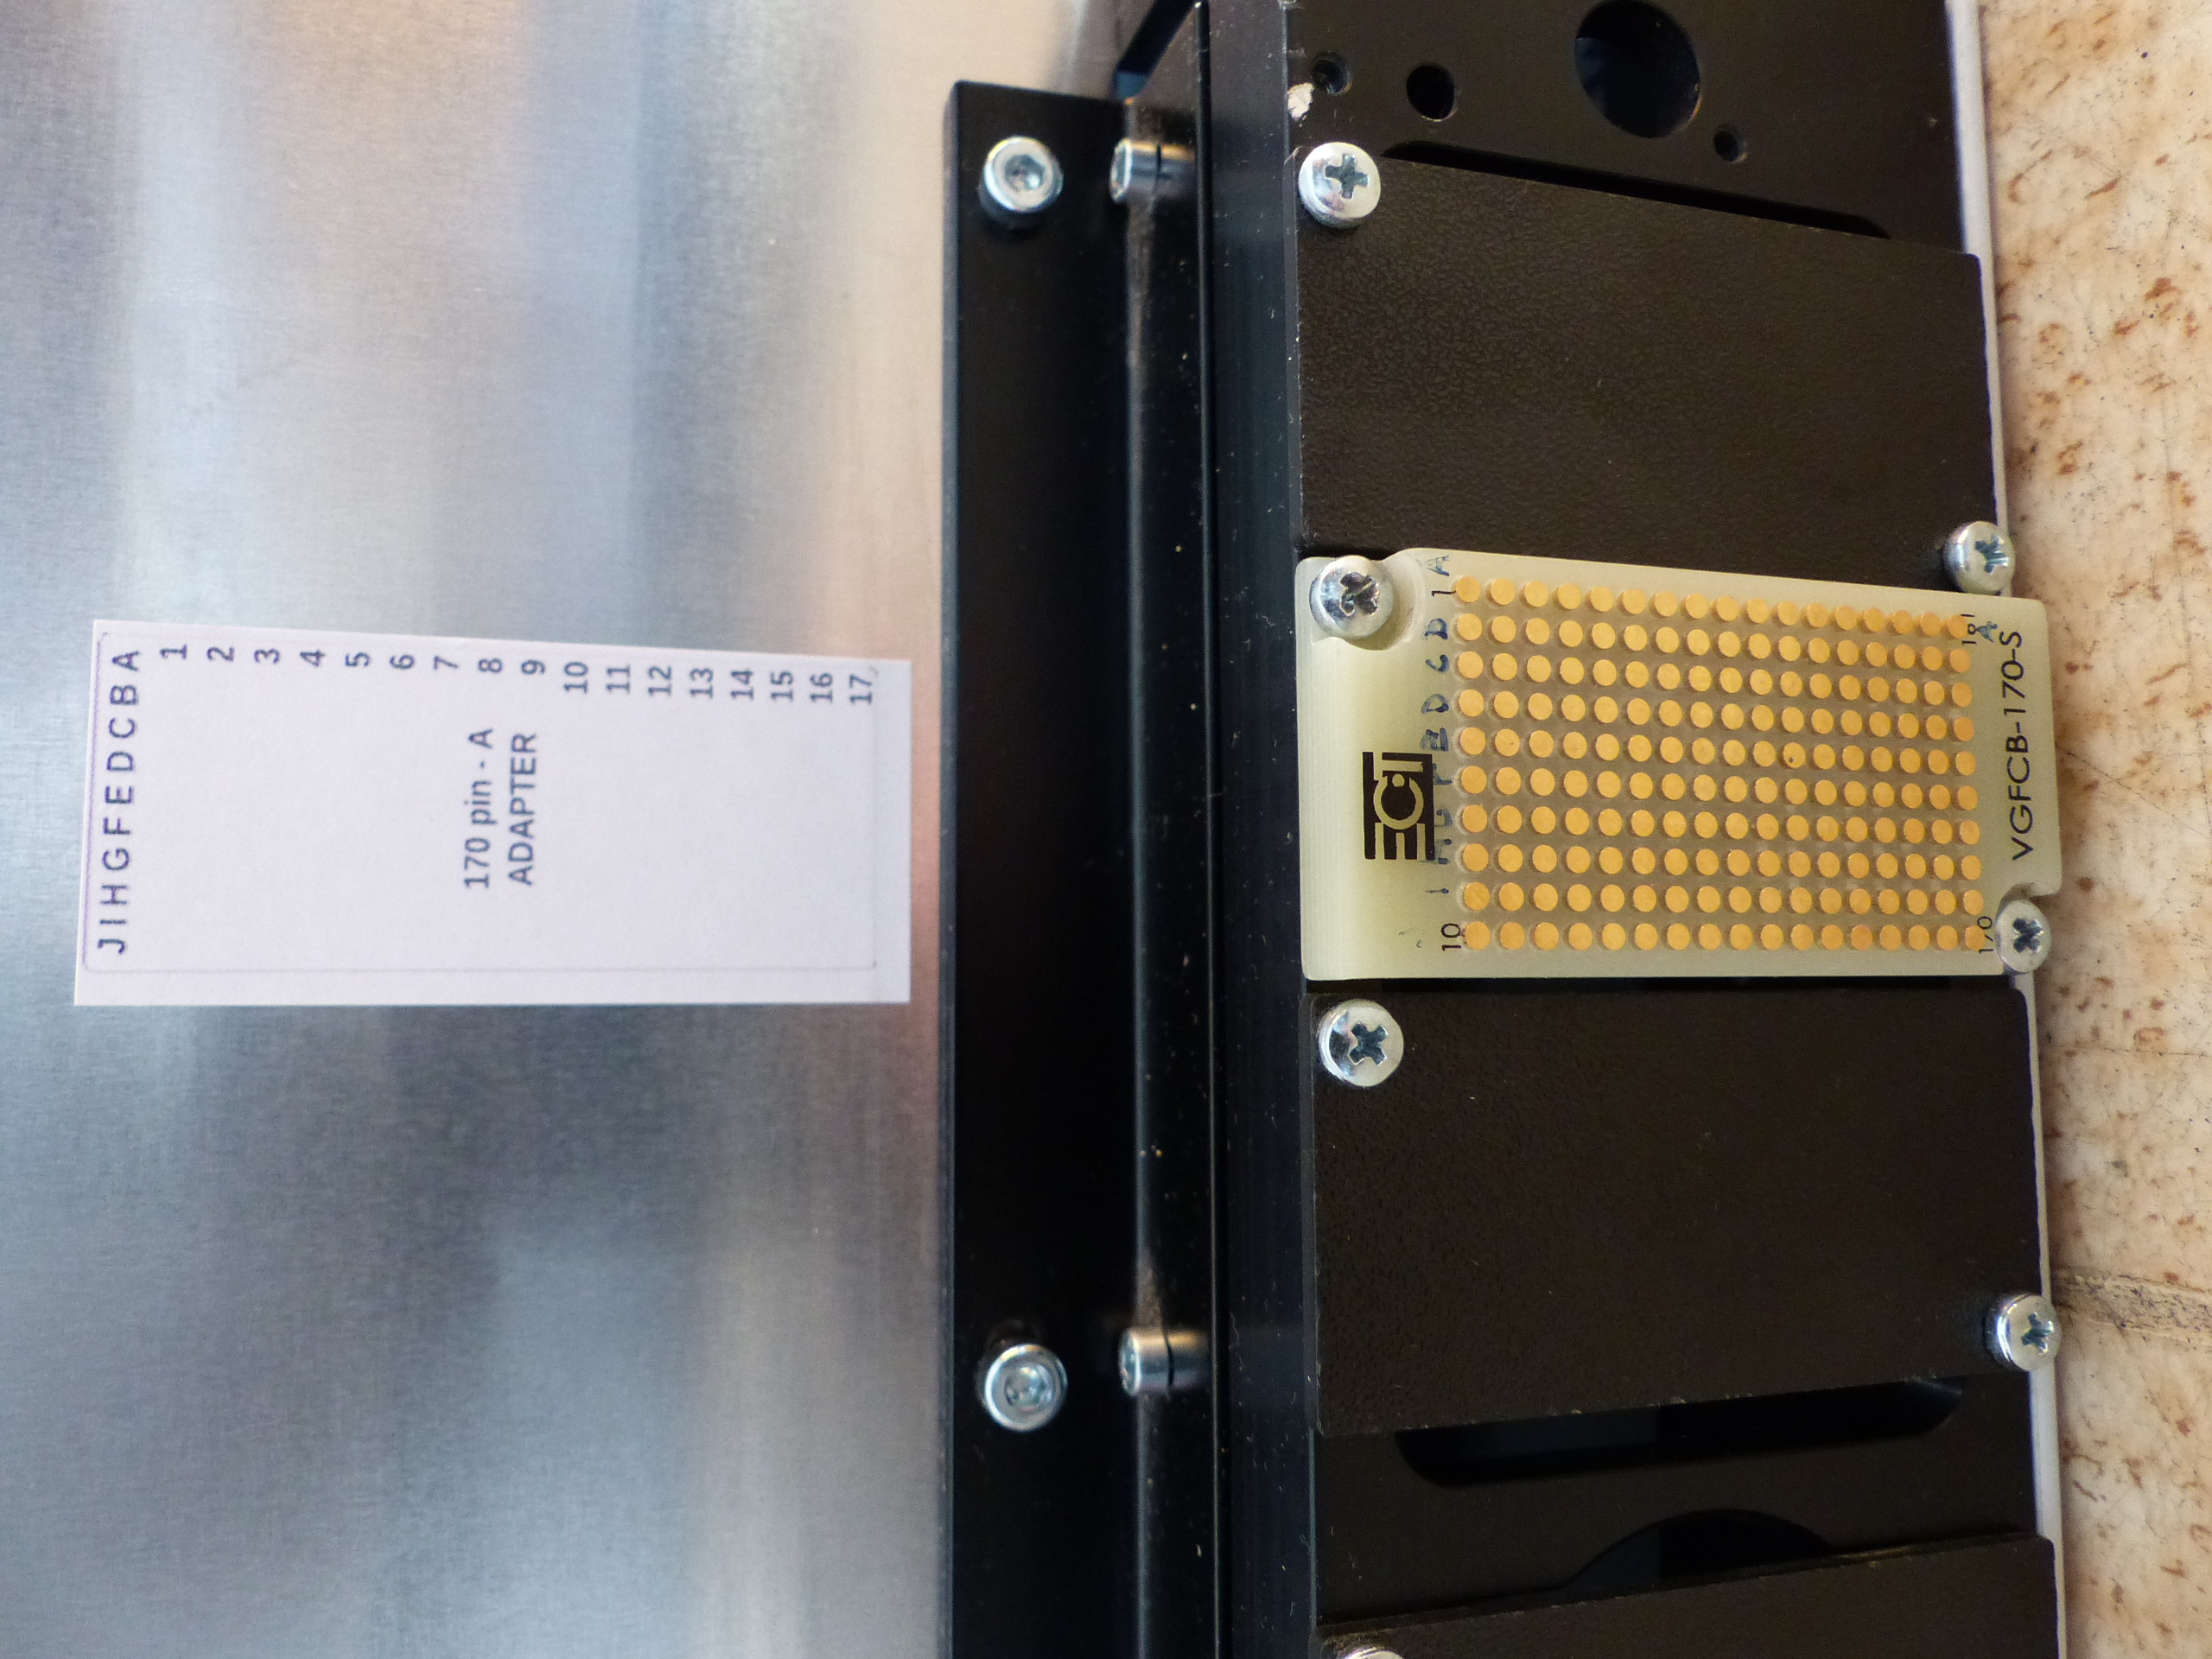
\includegraphics[width = \textwidth, angle = -90]{obrazky/170pin.JPG}
			\caption{Propojovací 170-ti pinový konektor}
		\end{minipage}
	\end{figure}


    \subsection{Výměna adaptérů:}
	Před výměnou adaptéru je doporučeno vypnout software a ujistit se, že neprobíhají žádné testy. Po vypnutí ovládacího 
	softwaru lze bezpečně stávající adaptér odebrat a připojit nový.\\


	\begin{minipage}{0.5\textwidth}
		\begin{enumerate}
			\item Pokud běží ovládací software, počkejte na dokončení testů a software vypněte.
			\item Odaretujte adaptér pomocí aretační páky
			\item Adaptér nadzvedněte tak, aby došlo k vyháknutí adaptéru z háků za které je zachycen.
			\item Do háků vložte nový adaptér
			\item Zaaretujte adaptér pomocí aretační páky
		\end{enumerate}
	\end{minipage}
	\hfill
	\begin{minipage}{0.4\textwidth}
		\begin{figure}[H]
			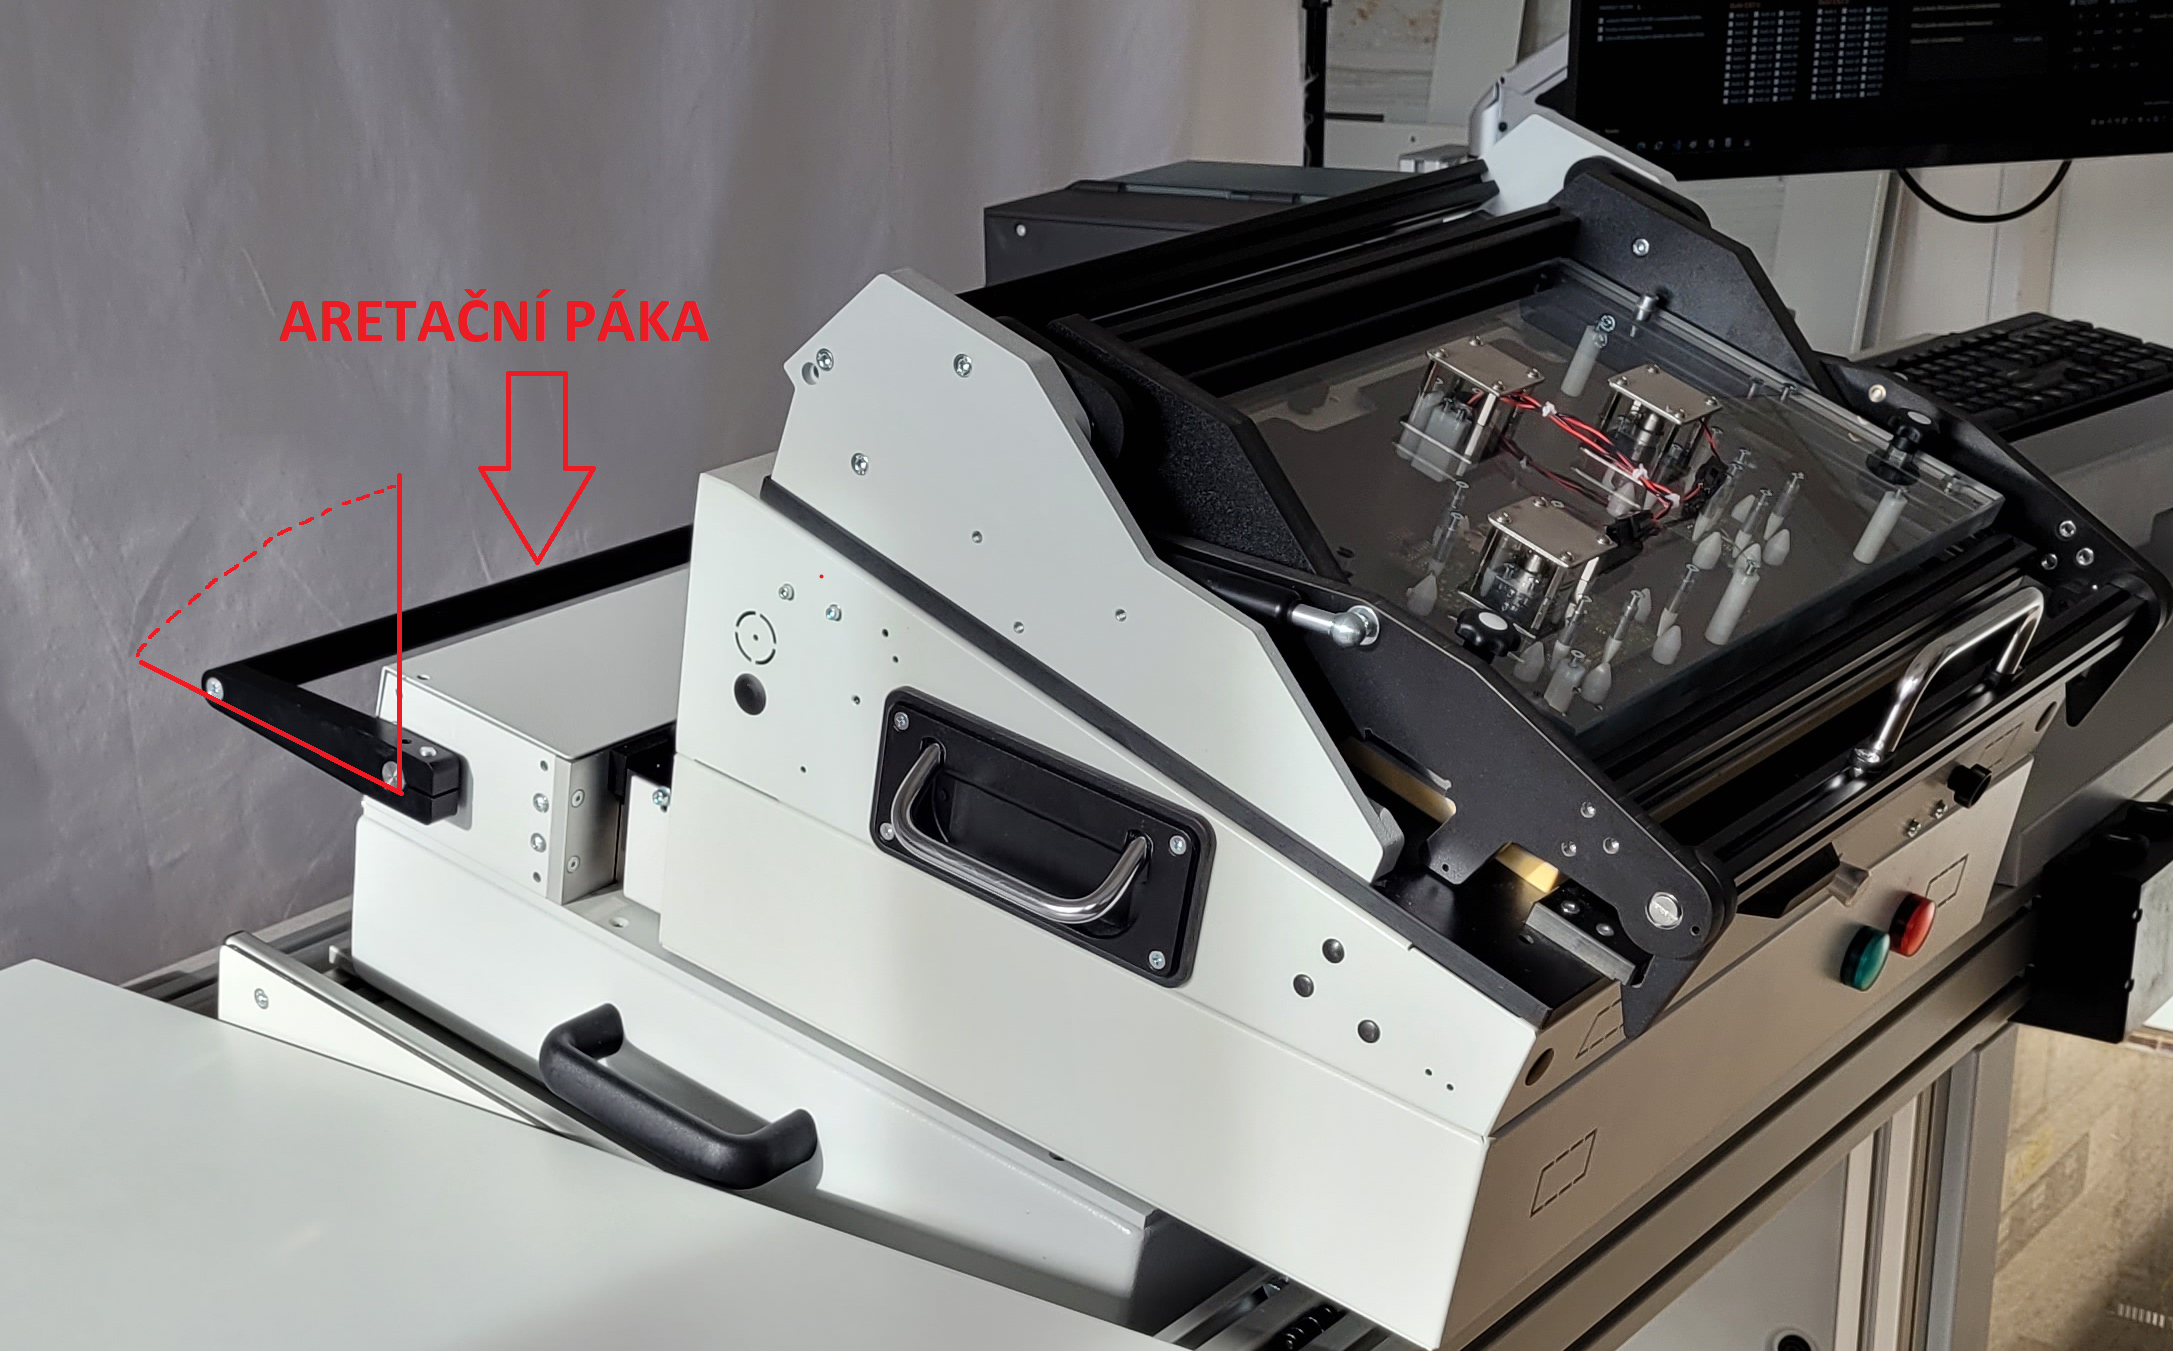
\includegraphics[width = \textwidth]{obrazky/aretacni_paka.png}
            \caption{Aretační páka}
		\end{figure}
	\end{minipage}

% 
\chapter{Obsluha zařízení:}
\section{Pracovní postup:}
	Pracovní postup by se dal shrnout do následujících bodů:

	\begin{enumerate}
		\item Přihlaste se pomocí přiložení uživatelské karty
		\item Naskenujte číslo zakázky
		\item Naskenujte Sériové číslo
		\item Vložte DUT do pozice zobrazené na monitoru\\
        Z důvodu snížení rizika opotřebení testovacích jehel je doporučeno vkládat do pozic, kde není připojena DUT záslepky viz. obrázek níže.
        \begin{figure}[ht!]
            \centering
            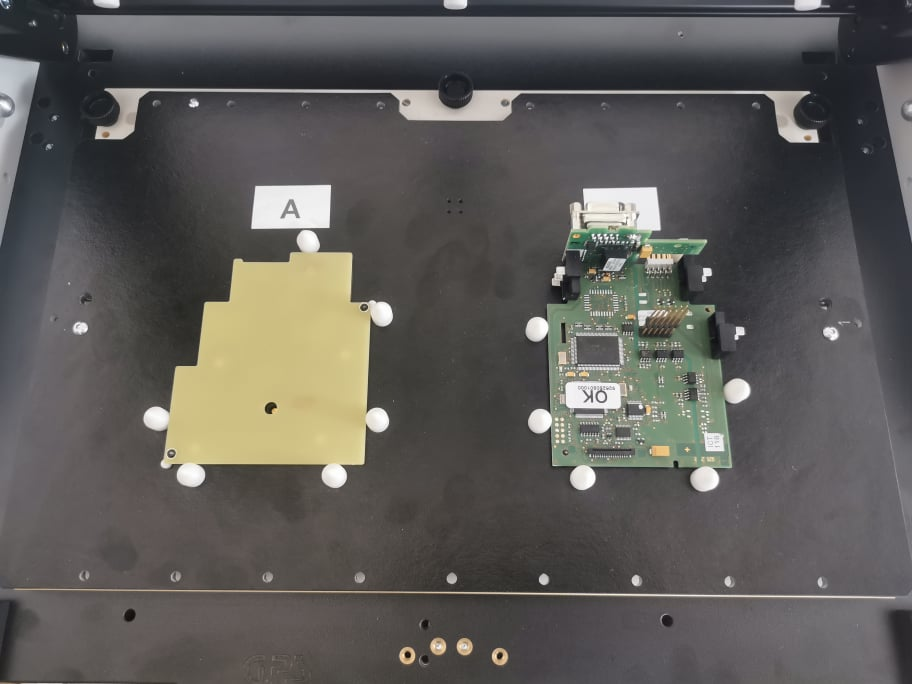
\includegraphics[width = 0.5\textwidth]{obrazky/adapt_zaslepka.jpg}
            \caption{Záslepky pro zakládání DUT do adaptéru}
        \end{figure}
    
		\item Počkejte na dokončení testu
		\item Vyjměte DUT
		\item Postup opakujte od bodu 3.
		\end{enumerate}

	Pro každý bod je obsluha vyzvána k příslušnému postupu pomocí textu na monitoru.
	Dále se může celý systém nacházet v různých chybových stavech. Pokud je chybový stav detekován,
	tak se na obrazovce monitoru zobrazí příslušná chybová hláška o vzniklé chybě a obsluha nebude moci provádět další testy
	až do odstranění chyby. Podrobnější informace naleznete v části SOFTWARE.

\chapter{Software}
Ovládací software lze používat v módu standardního a Admin uživatele.
Mezi jednotlivými módy se lze přepínat buď přiložením Administrátorské RFID karty a nebo
přihlášením pomocí jména "ADMIN" a příslušného hesla. Následující část je věnována módu standardního uživatele.
\section{Standardní uživatel}
Po spuštění programu se zobrazí následující obrazovka.
Program je rozdělen do dvou hlavních sekcí "Volba testované desky" a  "Tester". Přestože je v softwaru 
jasně viditelné logo SIEMENS, z důvodu posedlosti firmy SIEMENS svými logy,
tak celý software byl vytvořen firmou Čevor Innovation a.s.

\begin{figure}[ht!]
	\centering
	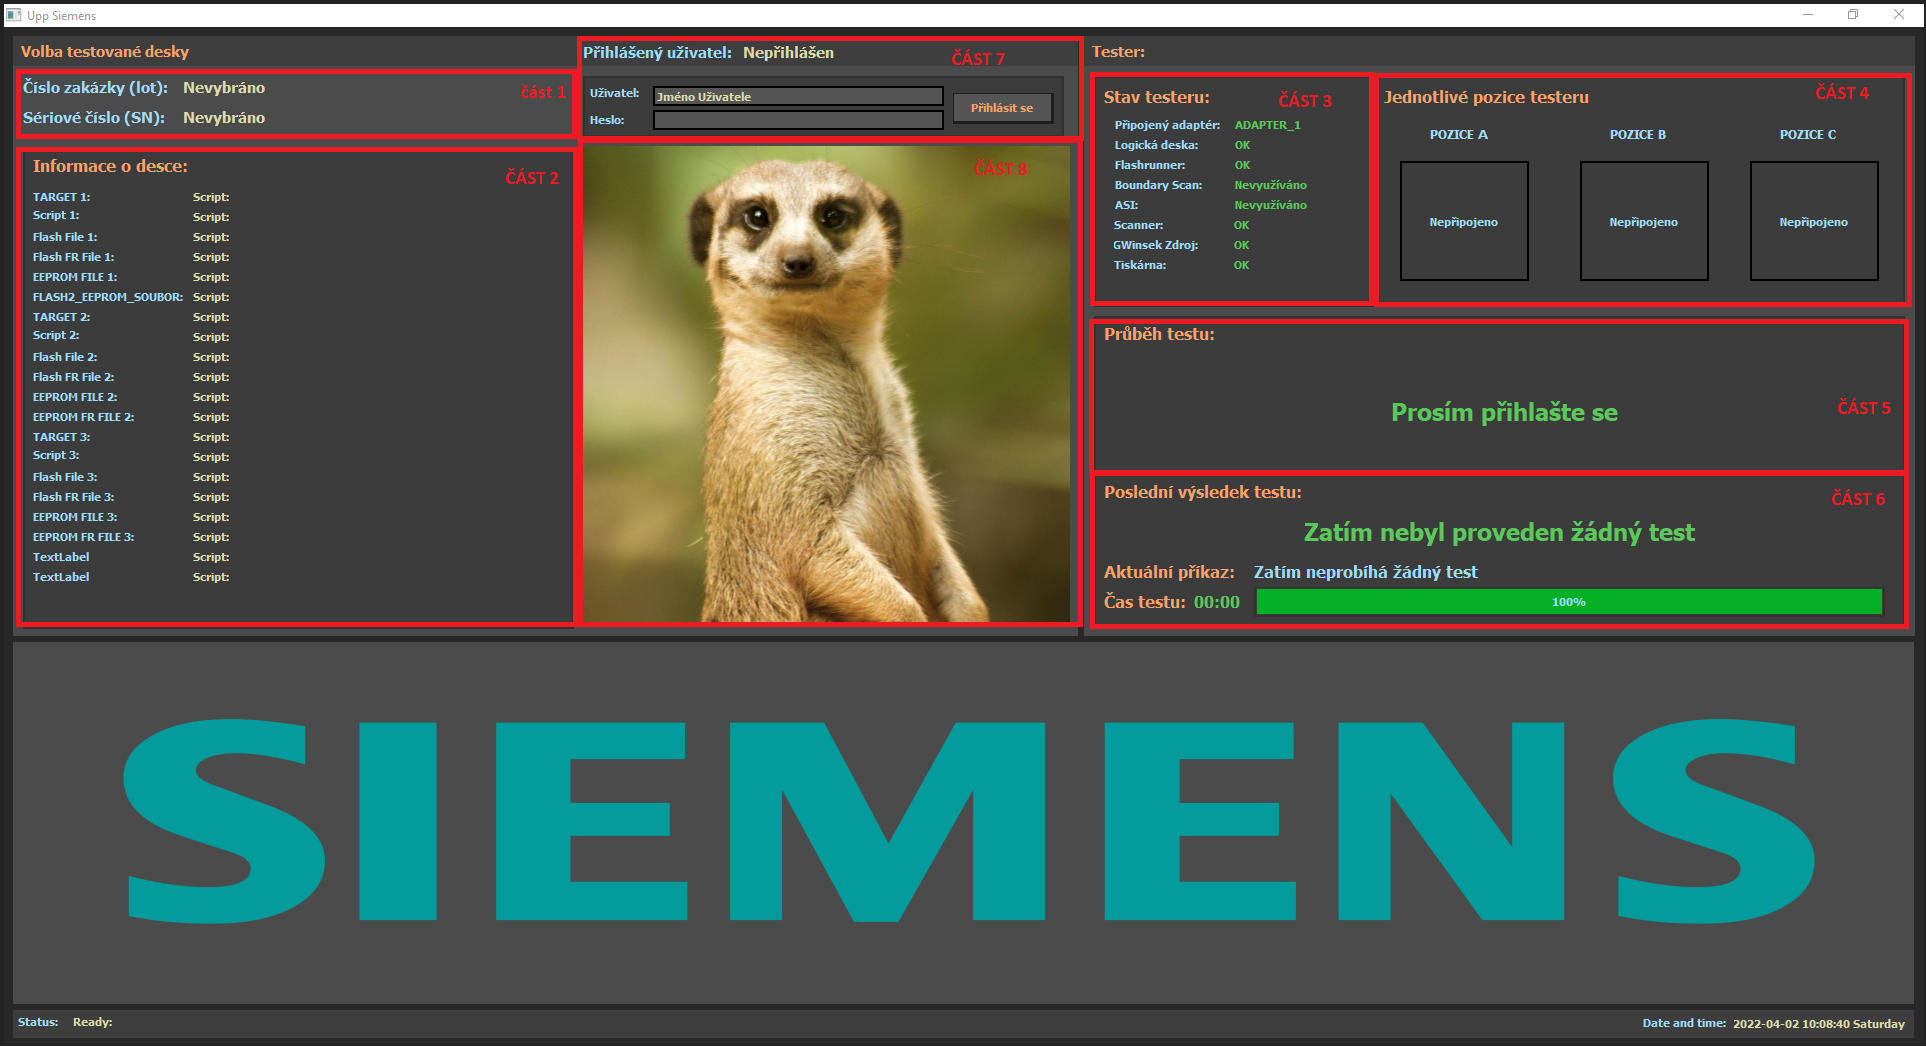
\includegraphics[width = 1\textwidth]{obrazky/LOGIN_EDITED.png}
    \caption{Obrazovka po spuštění programu}
\end{figure}

\subsection{Sekce volba testované desky}
V této sekci jsou zobrazeny v části 1 a 2. informace o právě zvoleném DUT (po zapnutí programu není vybráno žádné DUT). V části 7 
lze nalézt informace o právě přihlášeném uživateli a v části 8. se po přihlášení a naskenování správného
kódu zobrazí foto pro zvolené DUT.

\subsection{Sekce Tester}
V této sekci se v části 3 nacházejí aktuální informace o stavu testeru.
Tester provádí kontinuálně sebekontrolu a výsledky se zobrazují v části 3.
V části 4 jsou zobrazeny jednotlivé pozice připojeného adaptéru, které zobrazují,
zda je nebo není připojena DUT. V části 5 a 6 jsou zobrazovány pokyny obsluze a výsledky aktuálního testu.
Po spuštění programu by se měl zobrazovat pokyn "Prosím přihlaste se".

\clearpage

\section{Software - Obsluha testeru}

\subsection{Přihlášení obsluhy}
Přihlášení obsluhy se provádí pomocí vložení uživatelské karty do slotu pro uživatelské karty. Případně je možné
se přihlásit správnou kombinací jména a hesla v části 7.
V případě, že dojde k přihlášení uživatele, který má v systému uloženou fotografii, tak se změní obrázek surikaty
na obrázek uživatele. V případě, že uživatel nemá uloženou fotografii, tak se bude uživatel muset spokojit
s obrázkem surikaty případně jiného zvířete. 
Po přihlášení by obsluha měla být vyzvána v části 5 k naskenování čísla zakázky.

\subsection{Skenování čísla zakázky:}
Na stole je umístěna ruční čtečka čárových kódů, pomocí které obsluha načte číslo zakázky.
Po načtení čísla zakázky by obsluha měla být vyzvána k naskenování Sériového čísla.

\section{Skenování Sériového čísla:}
Po naskenování čísla zakázky by už měly být dostupné informace o DUT
(foto a informace v levé části programu na Obr.\ref{fig: informace o DUT})
\begin{figure}[ht!]
	\centering
	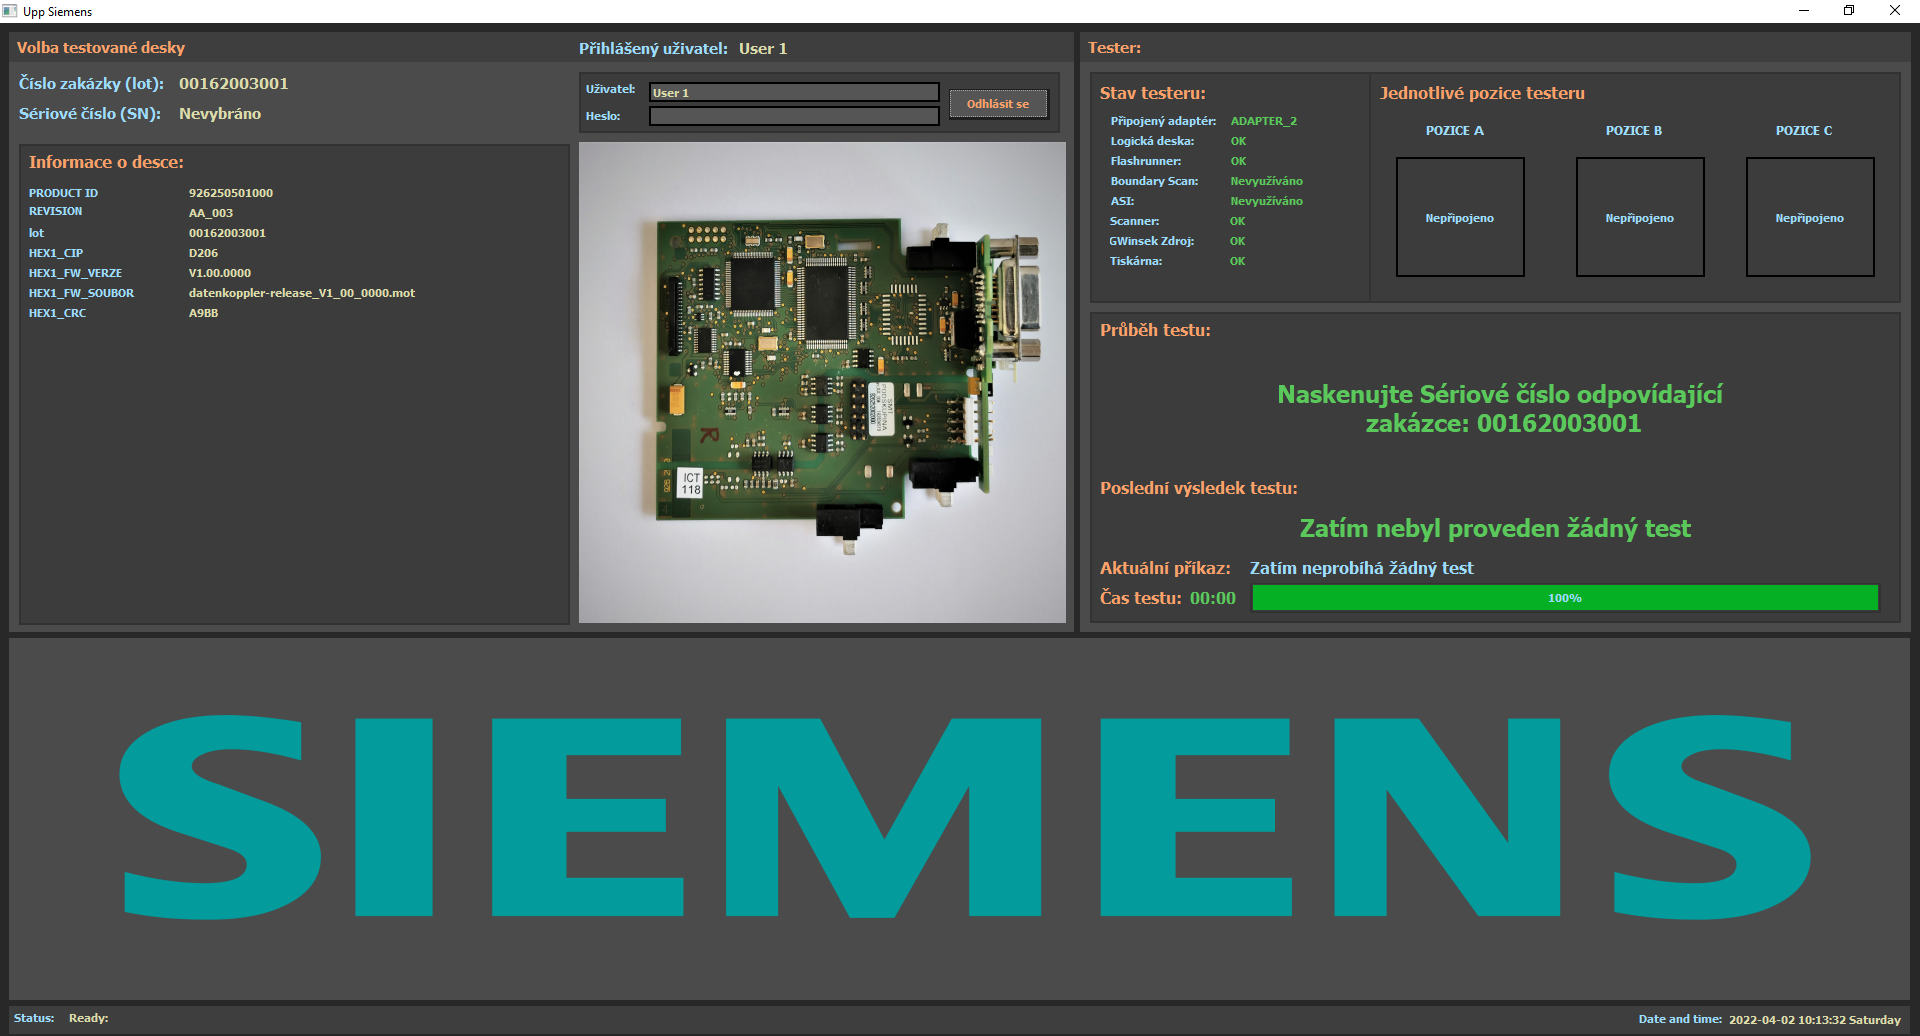
\includegraphics[width = 1\textwidth]{obrazky/SCAN_SN.PNG}
    \caption{Informace o DUT}
    \label{fig: informace o DUT}
\end{figure}

Obdobně jako při skenování čísla zakázky naskenuje obsluha sériové číslo.
Po načtení sériového čísla by obsluha měla být vyzvána k vložení DUT do správné pozice.
V případě, že DUT nemá sériové číslo je možné povolit testování bez sériového čísla v módu ADMIN.

\clearpage
\subsection{Vložení desky do správné pozice:}
Obsluha je nyní vyzvána k založení desky do pozice X a zavření víka.
Zde je navíc graficky znázorněno v části "Jednotlivé pozice testeru", kam má obsluha desku vložit.
Zde může nastat několik různých situací.

\begin{figure}[ht!]
	\begin{minipage}{0.32\textwidth}
		\textbf{Žádné DUT není založeno:}\\\\
		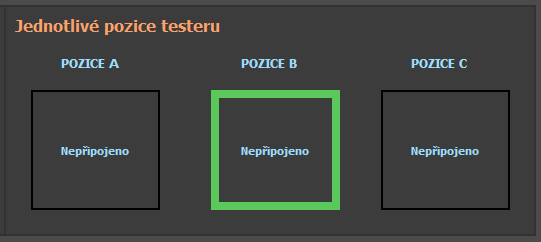
\includegraphics[width = 0.9\textwidth]{obrazky/NO_BOARD.PNG}
		
	\end{minipage}
    \hfill
	\begin{minipage}{0.32\textwidth}
		\textbf{DUT je založeno správně:}\\\\\\
		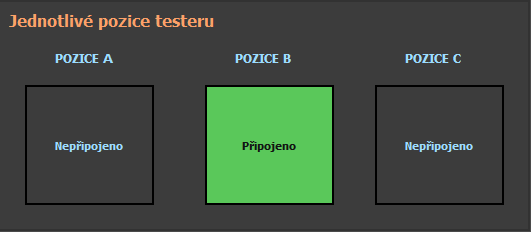
\includegraphics[width = 0.9\textwidth]{obrazky/OK_BOARD.PNG}
		
	\end{minipage}
    \hfill
	\begin{minipage}{0.32\textwidth}
		\textbf{DUT je založeno nesprávně:}\\\\
		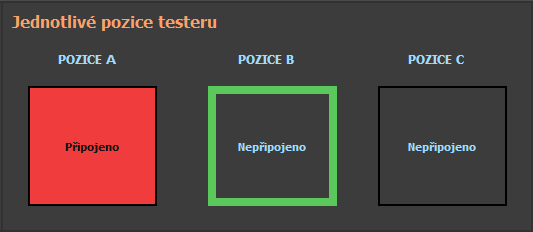
\includegraphics[width = 0.9\textwidth]{obrazky/BAD_BOARD.PNG}
		
	\end{minipage}
    \caption{Identifikace správné pozice DUT}
\end{figure}

Po vložení desky do správné pozice, spustí se testovací procedura pro zvolené DUT
a obsluha je vyzvána k čekání na dokončení testu.
Průběh testu je možno sledovat zde:
\begin{figure}[ht!]
	\centering
	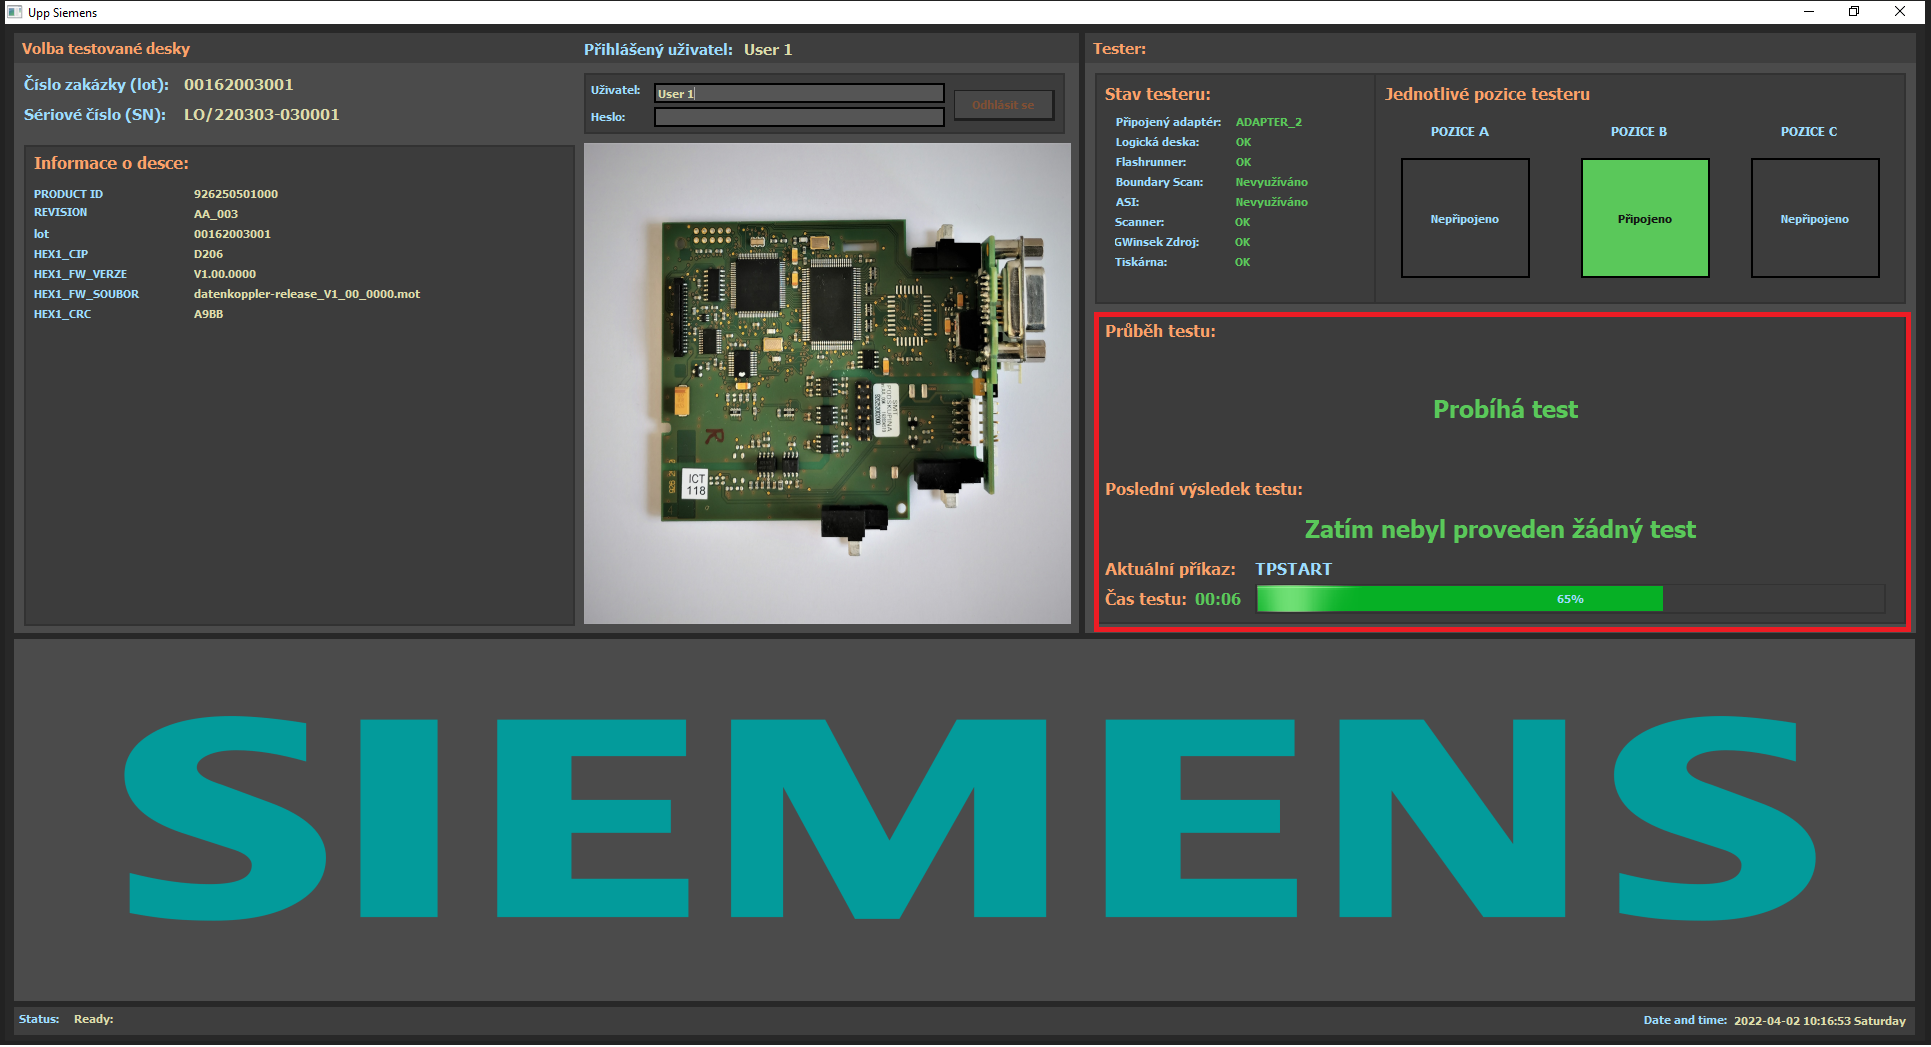
\includegraphics[width = 1\textwidth]{obrazky/TEST_START_EDITED.PNG}
    \caption{Průběh testu}
\end{figure}

\clearpage
\subsection{Dokončení testu:}
Po dokončení testu je v závislosti na výsledku testu obsluha informována o dalším postupu.

\begin{enumerate}
	\item \textbf{Test byl dokončen s výsledkem PASS:}
	\begin{figure}[ht!]
		\centering
		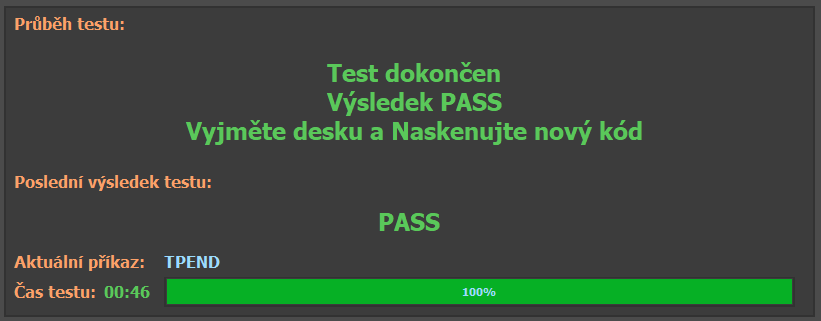
\includegraphics[height = 0.2\textheight]{obrazky/PASS_EDITED.PNG}
	\end{figure}

	\item \textbf{Test byl dokončen s výsledkem FAIL:}
	\begin{figure}[ht!]
		\centering
		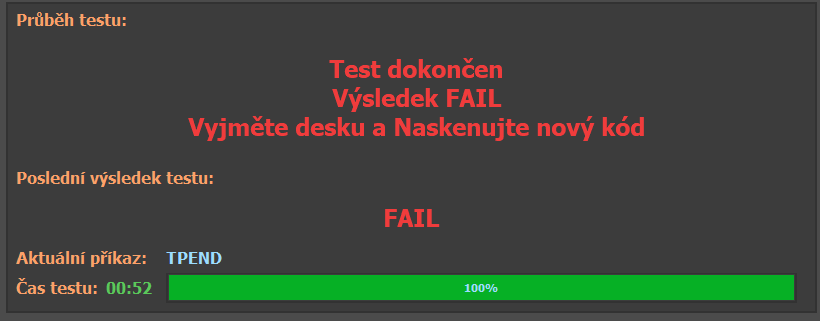
\includegraphics[height = 0.2\textheight]{obrazky/FAIL_EDITED.PNG}
	\end{figure}

	\item \textbf{Víko bylo otevřeno před dokončením testu:}
	\begin{figure}[ht!]
		\centering
		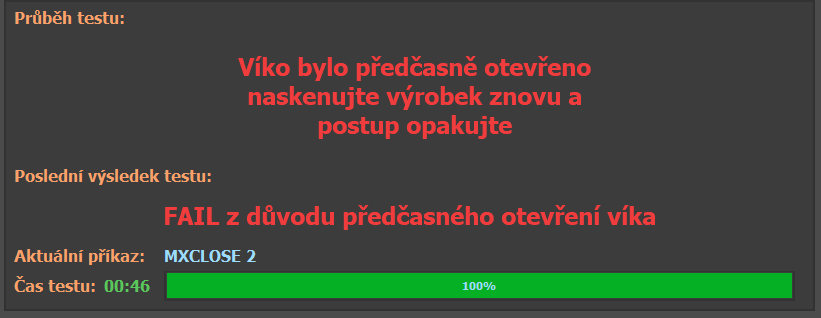
\includegraphics[height = 0.2\textheight]{obrazky/COVER_EDITED.PNG}
	\end{figure}

	V případě PASS a FAIL se nahraje výsledek do EMES (webová služba, kterou SIEMENS používá k ukládání dat)
    a podrobný log se uloží lokálně na cestu,
	která je odeslána do EMES a vytiskne se příslušný štítek.
	V případě FAIL z důvodu předčasného otevření víka nedojde k odeslání logu do EMES a Sériové číslo lze opět naskenovat.
	Poté je obsluha vyzvána k odebrání desky a naskenování nového kódu.

\end{enumerate}

\clearpage
\section{Paralelní programování}
Po naskenování určitých zakázek se program přepne do paralelního módu.
V tomto módu je možné naskenovat více sériových čísel a programovat tak DUT ve více pozicích najednou. Obsluha je instruována následovně:\\
\subsection{Skenování pozice A:}
V tomto bodě je obsluha k naskenování sériového čísla odpovídající DUT, které se bude zakládat do \mbox{pozice A.}
	\begin{figure}[ht!]
		\centering
		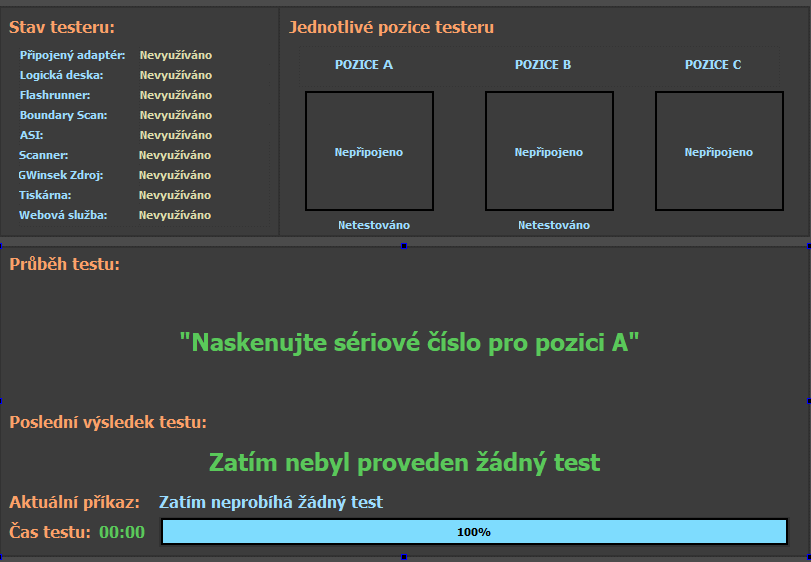
\includegraphics[height = 0.22\textheight]{obrazky/dual_SCAN_A.PNG}
        \caption{Skenování pozice A}
	\end{figure}

\subsection{Skenování pozice B:}
	V tomto bodě je obsluha vyzvána k naskenování sériového čísla odpovídající DUT, které se bude zakládat do pozice B. V případě,
	že obsluha chce otestovat pouze DUT v pozici A, může tento krok přeskočit a přímo vložit DUT do pozice A a zavřít víko.
	Po zavření víka je automaticky zkontrolováno, zda je DUT opravdu založeno do pozice A a začne test.
    Zároveň je obsluha graficky informována v části "jednotlivé pozici testeru"
    o stavu jednotlivých pozic. Grafické vyhodnocení je obdobné jako při neparalelním programování
    v sekci "Vložení desky do správné pozice".
	\begin{figure}[ht!]
		\centering
		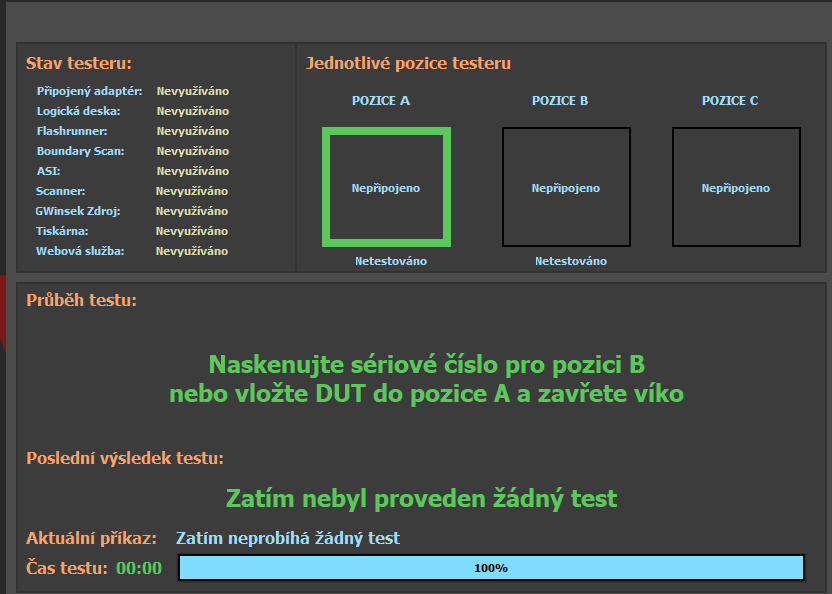
\includegraphics[height = 0.22\textheight]{obrazky/dual_SCAN_B.PNG}
        \caption{Skenování pozice A}
	\end{figure}


\subsection{Průběh testu:}
Po úspěšném založení DUT a zavření víka se spustí jednotlivé testy. Zároveň se změní popisky v části "Jednotlivé pozice testeru"\ následovně:
	\begin{figure}[ht!]
		\centering
		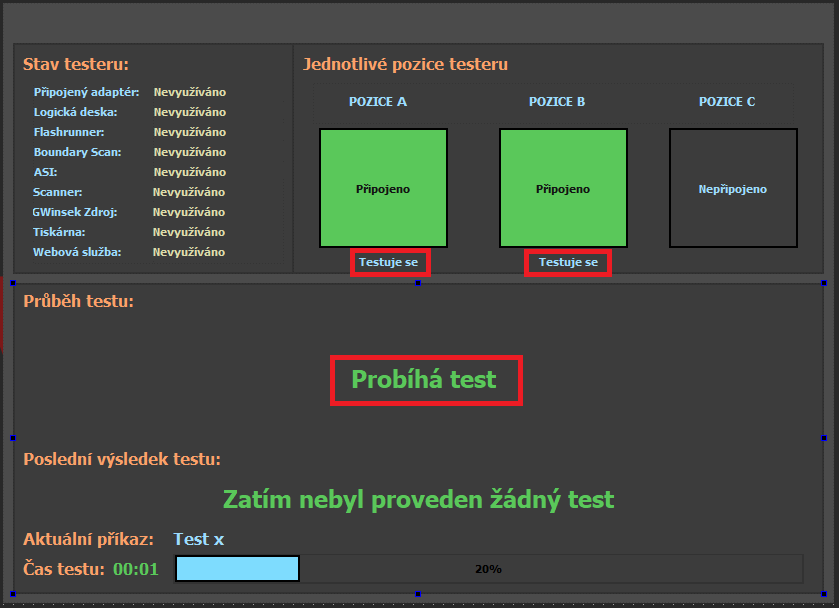
\includegraphics[height = 0.35\textheight]{obrazky/dual_SCAN_TEST.PNG}
        \caption{Průběh testu - paralelní programování}
	\end{figure}

\subsection{Výsledky testů:}
Výsledek testů je pak zobrazen pro jednotlivé pozice jak v části "Jednotlivé pozice testeru", tak v části "Průběh testu".
	\begin{figure}[ht!]
        \begin{minipage}{0.49\textwidth}
        \centering
		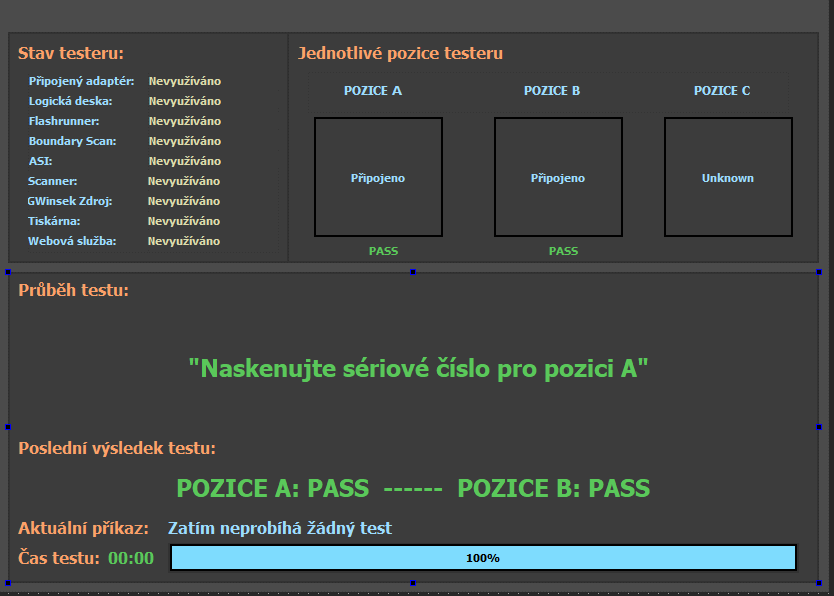
\includegraphics[height = 0.22\textheight]{obrazky/dual_SCAN_PASS.PNG}
        \caption{Výsledky testu - paralelní programování (PASS,PASS)}
        \end{minipage}
        \hfill
        \begin{minipage}{0.49\textwidth}
            \centering
            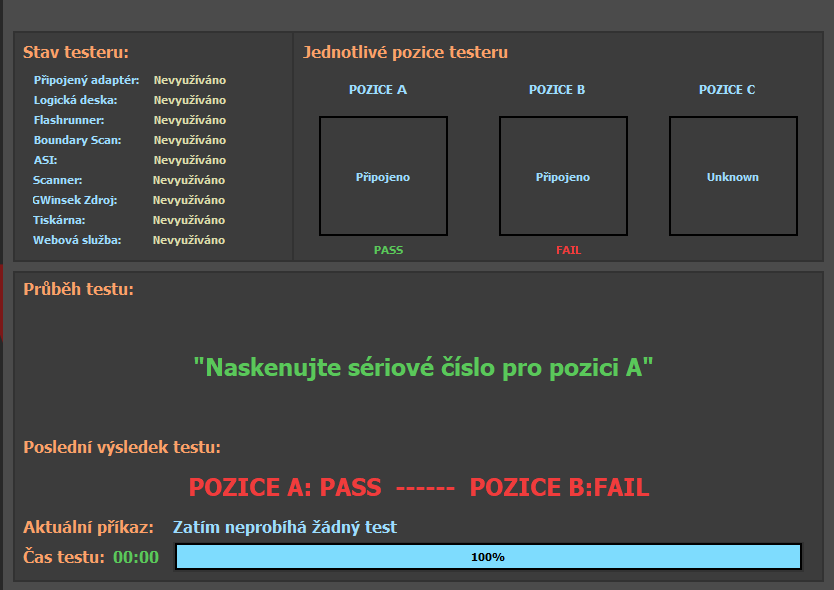
\includegraphics[height = 0.22\textheight]{obrazky/dual_SCAN_FAIL.PNG}
            \caption{Výsledky testu - paralelní programování (PASS,FAIL)}
            \end{minipage}
	\end{figure}


\clearpage
\section{Testování LED}
Pro některá DUT je implementováno manuální testování LED. V případě, že je takový test implementován, zobrazí
se obsluze následující dialog:
\begin{figure}[ht!]
	\centering
	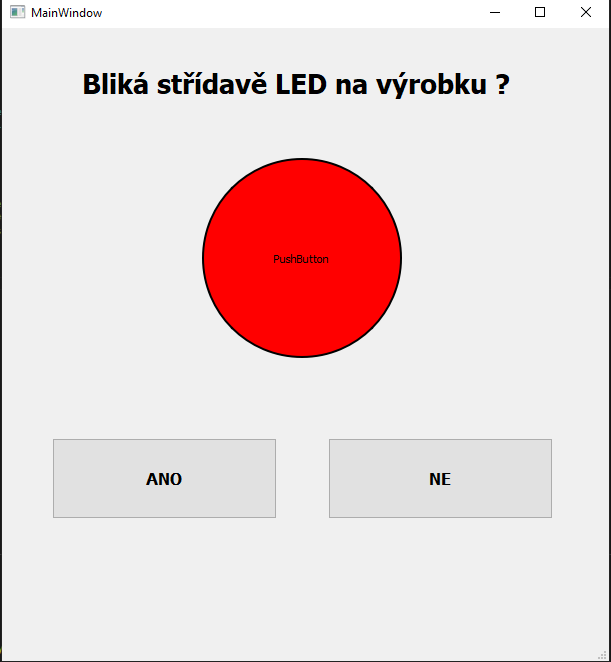
\includegraphics[width = 0.65\textwidth]{obrazky/LED_test.PNG}
    \caption{Testování LED}
\end{figure}

Obsluha zkontroluje, zda blikají/svítí příslušné LED a výsledek testu potvrdí kliknutím na tlačítko ANO popř. NE.
\clearpage
